\chapter{Results and interpretation}\label{chap:results}
Now that all backgrounds are well estimated, the background prediction works fine in the validation region, and all uncertainties are determined, the background prediction can be applied to the SR, $\ptmiss>150\GeV$ and $\mtTwo>100\GeV$, and predicted and observed event counts can be compared. An excess or other significant deviations from the prediction would be indicators for BSM physics.
\section{Results}\label{sec:results}
\subsection*{Signal region binning}
In order to perform the counting experiment, a distinct binning in one or multiple variables needs to be applied to the SR. This binning can be optimized considering different criteria, \eg observation and exclusion power. Since the most sensitive variables are $\ptmiss$ and $\mtTwo$, different one dimensional and two dimensional binnings are trialed. For individual benchmark points of all three signal models, simplified significances $\frac{s}{s+b}$, where s is the number of signal events and b the number of background events per bin, the binnings are varied. Because the total predicted event count in the SR is of the order of $13$ events, special care has to be taken regarding this issue. Albeit many sensitive bins with lower SM prediction and high signal expectation would push expected exclusion limits, this would make reinterpretations and observations difficult due to the high statistical uncertainties of the measured data.\\
To take into consideration all those aspects, a binning consisting of two bins in the $\ptmiss$ distribution are chosen, as already introduced in \refSec{sec:SRSelection}. The first bin starts at $150\GeV$ and ends at $200\GeV$, while the second one is an overflow bin, meaning all events with $\ptmiss>200\GeV$ in the SR are counted in that bin. This binning yields on the one side good exclusion power, because the $\ptmiss$ distribution is observed to be more sensitive than the $\mtTwo$ distribution, and on the other side includes an amount of events large enough in each bin, so that the reinterpretation is not restricted by statistical uncertainties. Due to the same reasons, two dimensional binnings are discarded.
\subsubsection*{Possible influence of signal to the validation region}
The SR and the VR are very close to each other in phase space due to the chosen sideband structure of the VR. Thus, some signal events, especially for low SUSY masses, are expected to populate also the VR. The distribution most sensitive to this effect is the $\pt^{\PGg}$ distribution of the selected photon, as shown in \refFig{fig:signalContVR}.
\begin{figure}[tbp]
 \centering
 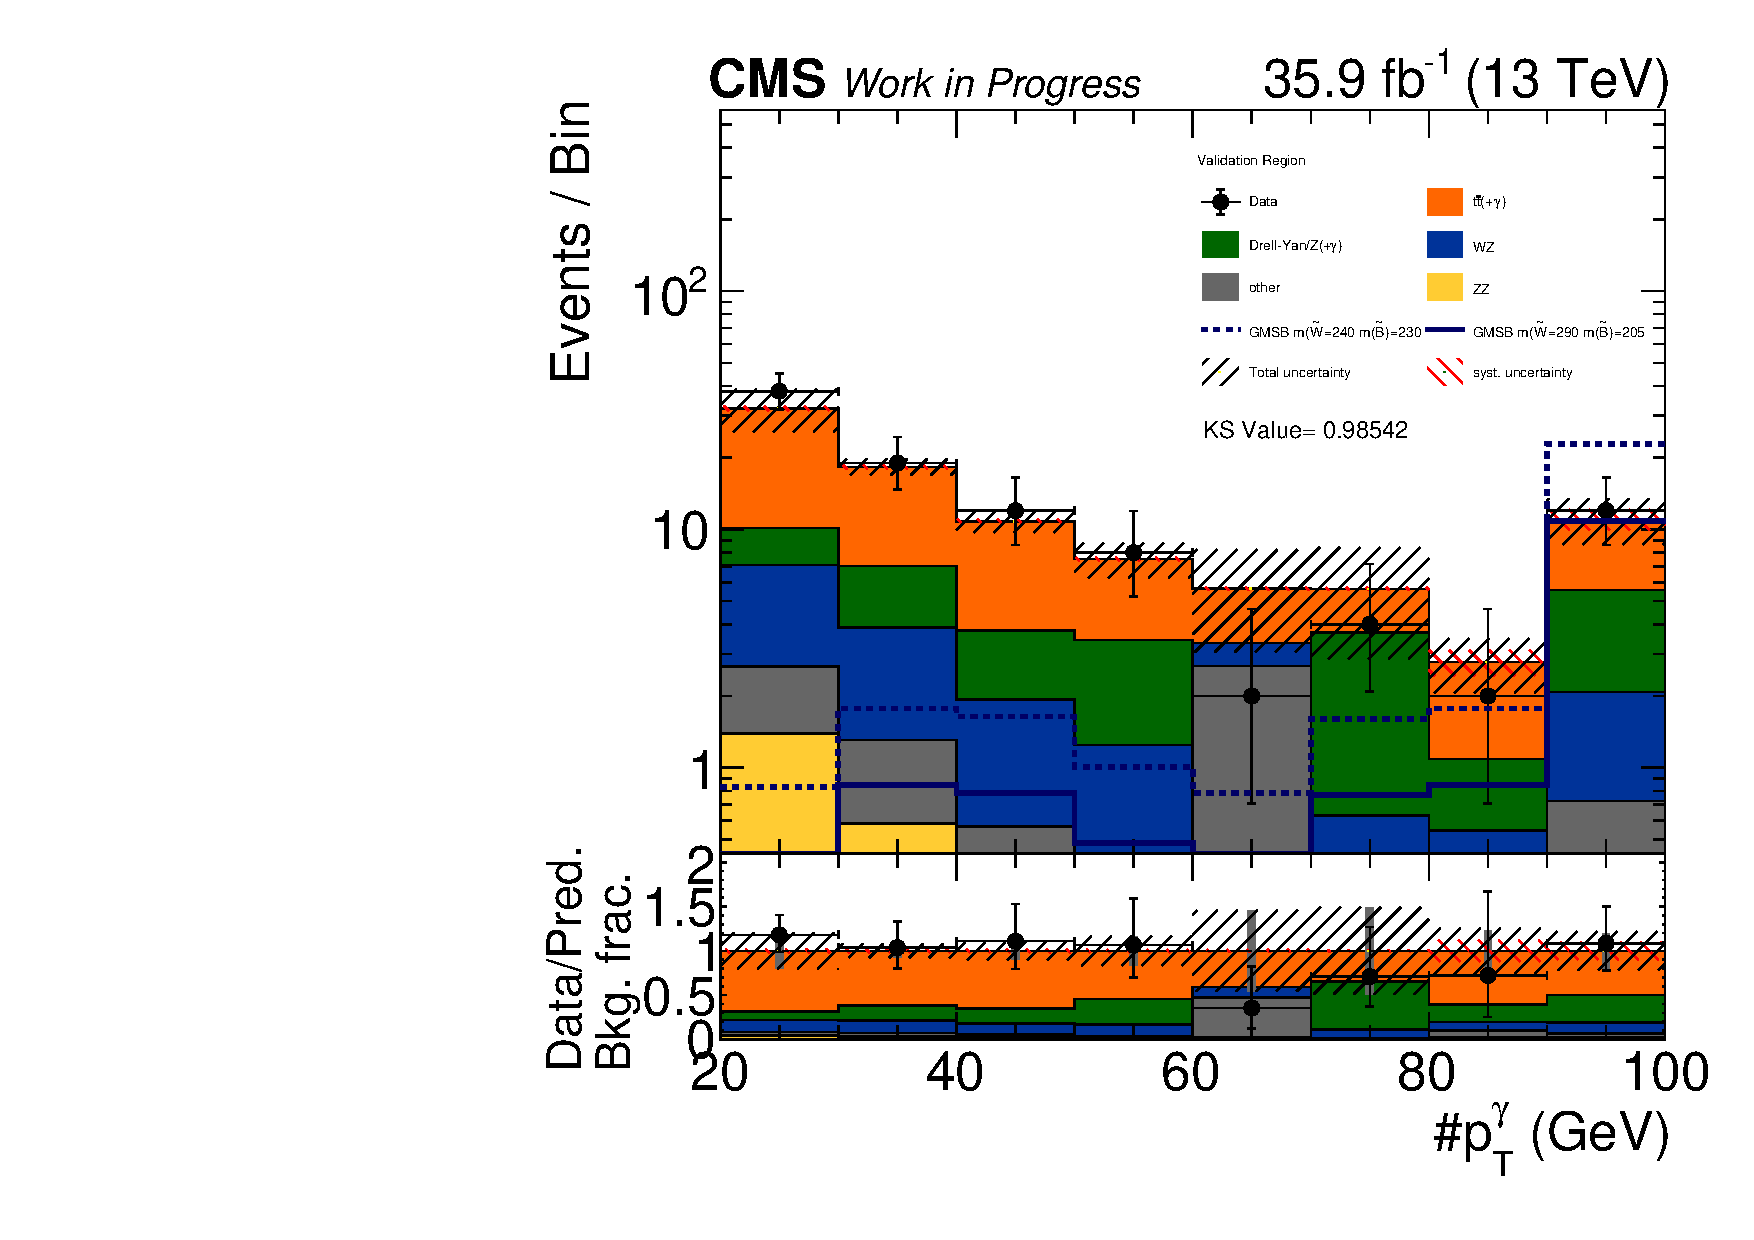
\includegraphics[width=\pairwidth]{figures/VR_signal_study/VR_LL_pt_g1_log}
 \caption{The transverse momentum distribution of the photon in the VR. Signal benchmark points are also added to show the possible sensitivity in the high $\pt^{\PGg}$ regime.}
 \label{fig:signalContVR}
\end{figure}
At high $\pt^{\PGg}$ ranges ($>80\GeV$), a considerable amount of signal events is measurable in the VR. Since the predicted background and observed data are already compared in the VR, and no background prediction is performed here, there is no need to account for this effect like in the other CR in terms of signal contamination.\\
Hence, the subtraction of this region from the VR, and the addition to the SR as a third search bin would increase the total sensitivity. But, because the number of expected signal events in the two SR bins is  already high enough for the relevant signal points, this strategy does not show any improvement in the overall sensitivity,+ that is large enough to justify the deterioration in the simplicity of the analysis.

\subsection{Event yields}
The final background prediction together with the observed event yield is shown in \refFig{fig:result}.
The total background uncertainties are obtained by adding the individual uncertainties quadratically. The statistical uncertainties on the measurement are calculated using $68\%$ confidence intervals of the Poisson distribution with the mean set to the observed yield.
To show the effect of a possible signal in the counting experiment, contributions of two example signal points are drawn for comparison. The measured data yields are in good agreement with the predicted background events, thus no evidence for BSM physics is found. The measured excess corresponds to a significance of $1.26\sigma$.
\begin{figure}[tbp]
 \centering
 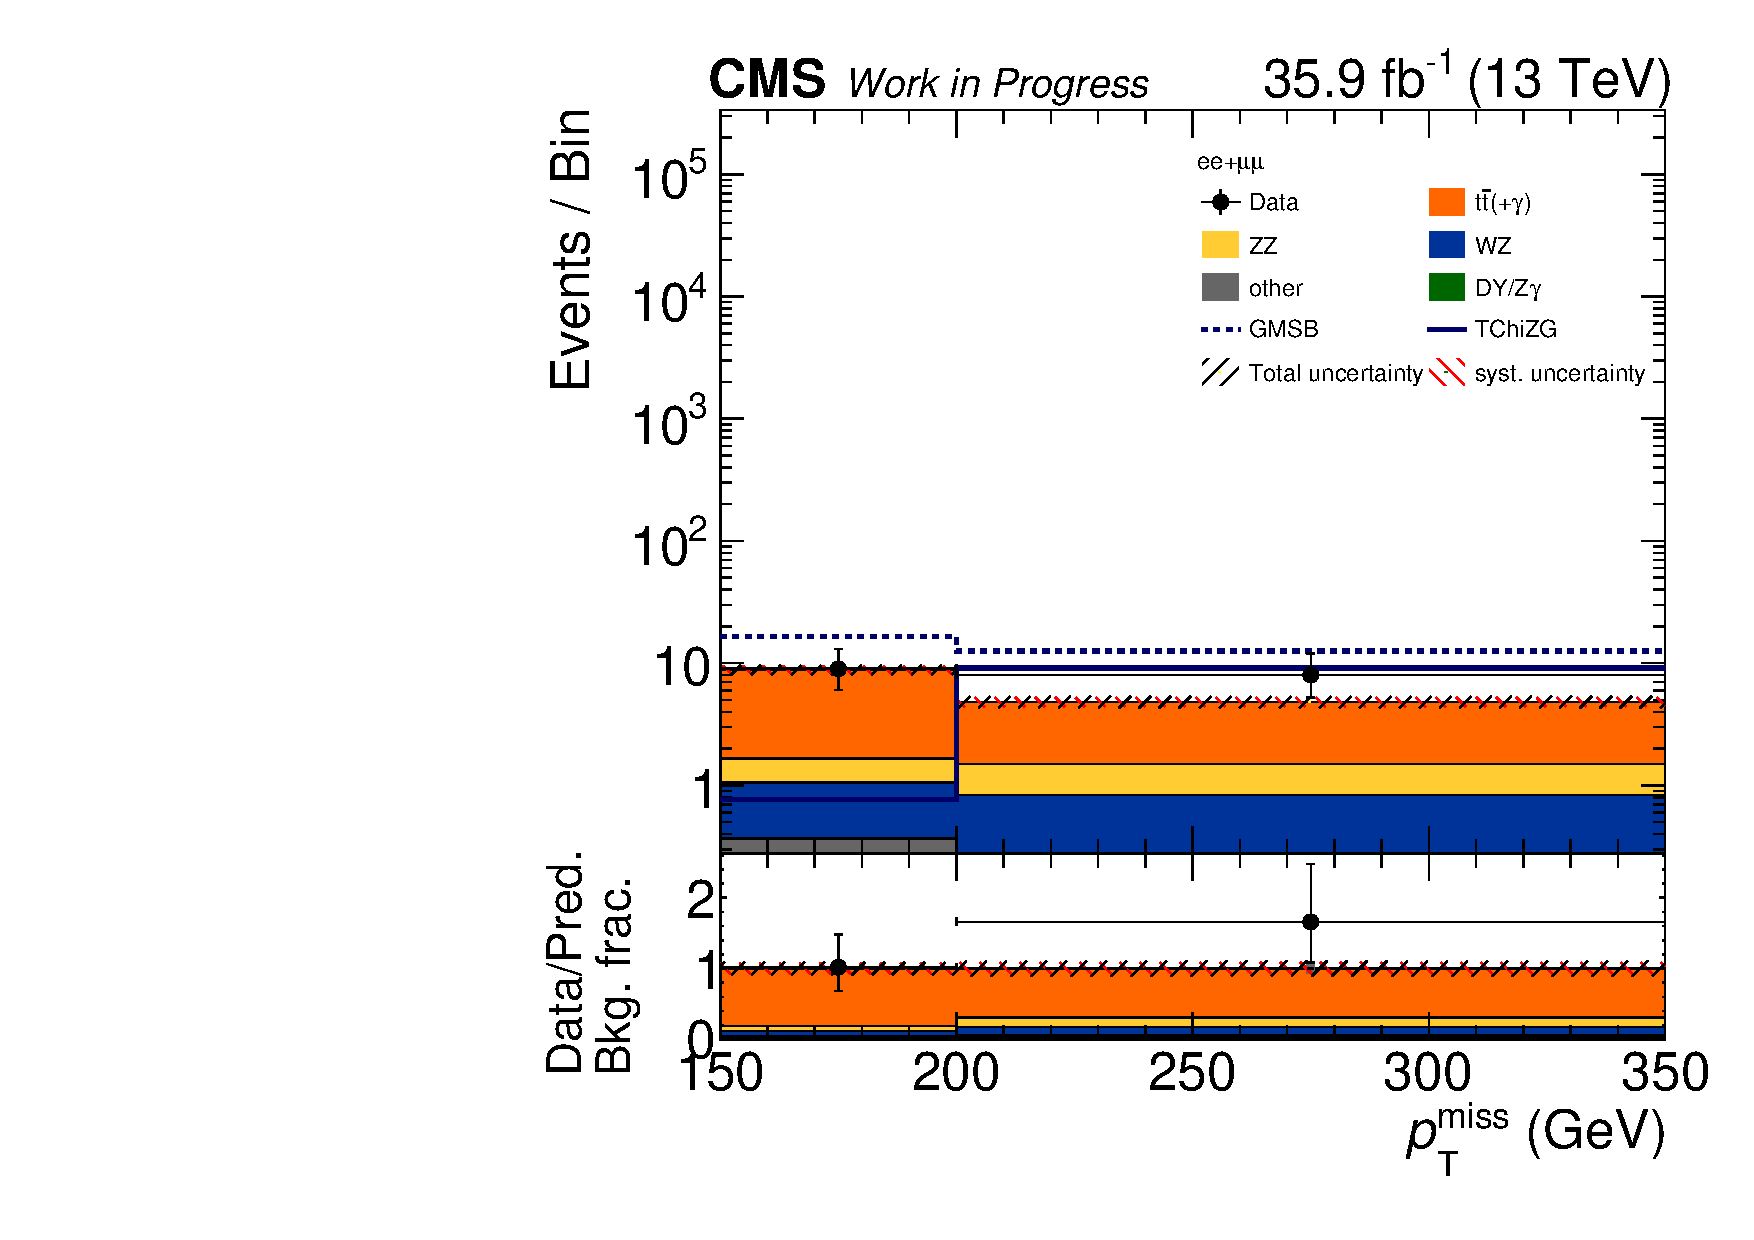
\includegraphics[width=\pairwidth]{figures/UnblindingPlots/final_MC_log}
 \caption{Comparison between final prediction and observation with statistical and systematic uncertainties in the signal region. Two signal expectations for the TChiZg model with $m(NLSP)=600\GeV$ and the GMSB model with $m(\tilde{W})=290\GeV$ and $m(\tilde{B})=205\GeV$ are also shown.}
 \label{fig:result}
\end{figure}
The number of background and observed events together with their total uncertainties are given also in \refTab{tab:results}.
\begin{table}[tbp]
 \centering
 \caption{Observed yields and final predicted background yields with the statistical and systematic uncertainties for each bin and background.}
 \normalsize
 \label{tab:results}
 \begin{tabular}{lllllll}
  $\ptmiss$      & \multicolumn{3}{l}{$150-200\GeV$} & \multicolumn{3}{l}{$200\GeV-\infinity$}                                                                  \\\hline
                 & yield                             & $\sigma_{stat}$                         & $\sigma_{syst}$ & yield & $\sigma_{stat}$    & $\sigma_{syst}$ \\\hline
  $\ttbar(\PGg)$ & 7.191                             & 0.316                                   & 0.664           & 3.320 & 0.229              & 0.395           \\
  DY/$\PZ(\PGg)$ & 0.152                             & 0.060                                   & 0.039           & 0.042 & 0.024              & 0.010           \\
  $\PW\PZ$       & 0.684                             & 0.081                                   & 0.063           & 0.579 & 0.076              & 0.054           \\
  $\PZ\PZ$       & 0.601                             & 0.019                                   & 0.052           & 0.667 & 0.020              & 0.061           \\
  Other          & 0.215                             & 0.215                                   & 0.191           & 0.214 & 0.214              & 0.108           \\\hline
  Total          & 8.843                             & 0.396                                   & 0.697           & 4.822 & 0.324              & 0.418           \\\hline
  Data           & 9                                 & $^{+4.11}_{-2.94}$                      & /               & 8     & $^{+3.95}_{-2.76}$ & /               \\\hline
 \end{tabular}
\end{table}


\section{Statistical interpretation}
No evidence for BSM physics is found, but the results can be interpreted in various SUSY models in terms of exclusion of available model parameter space.
\subsection{Limit calculation}
Upper cross section limits are calculated for signal points in the parameter space of simplified models with both electroweak and strong production, and a consistent GMSB model, as introduced in \refSec{sec:SMS}. All limits are calculated using modified frequentist $CL_s$ approach~\cite{CLS1,CLS2,CLS3} with a likelihood test statistics and asymptotic formulae~\cite{AsymptoticFormulae} at a confidence level (CL) of $95\%$. The compatibility of the background only ($b$) and signal plus background ($s+b$) hypotheses with the results is tested. Therefore, the signal strength modifier $\mu$ is introduced, in order to express both hypotheses in a uniform way $\mu s+b$, where $\mu=0$ yields the background only hypotheses, and $\mu>0$ corresponds to the $s+b$ hypotheses.\\
To account for systematic uncertainties, for each signal or background uncertainty a nuisance parameter $\theta$ is introduced, and signal and background yield are rewrote as functions of $\theta$: $s(\theta)$ and $b(\theta)$. Different probability density functions (pdf) $p(\tilde{\theta}|\theta)$ are also implemented in the likelihood, to reflect degree of belief in the true value of the nuisance parameter $\theta$, where $\tilde{\theta}$ is the default value of the nuisance parameter. Different pdfs are used to describe the uncertainties, such as the log normal or log uniform distributions. The total likelihood function $\mathcal{L}(data|\mu,\theta)$ reads
\begin{equation}
 \mathcal{L}(data|\mu,\theta)= Poisson(data|\mu\cdots(\theta+b(\theta))\cdot p(\tilde{\theta}|\theta)).
\end{equation}
Here, $data$ represents the actual experimental observation, and $Poisson(data|\mu\cdots(\theta+b(\theta))$ stands for the probability to observe $n_i$ events in $i$ bins:
\begin{equation}
 \prod_i \frac{(\mu s_i+b_i)^{n_i}}{n_i!}e^{-\mu s_i - b_i}.
\end{equation}
A test statistics $\tilde{q_\mu}$ is introduced as a likelihood ratio, because according to the Neyman-Pearson Lemma this is the discriminator suited best for the testing of two alternative statistical hypotheses while minimizing the rate of wrongly rejected true hypotheses and accepted false hypotheses:
\begin{equation}
 \tilde{q}_{\mu}= -2 \ln \frac{\mathcal{L}(data|\mu,\hat{\theta}_{\mu})}{\mathcal{L}(data|\hat{\mu},\hat{\theta})}, \,\mathrm{with}\,0\leq\hat{\mu}\leq\mu.
\end{equation}
Here, $\hat{\theta}_{\mu}$ refers to the conditional maximum likelihood estimators of $\theta$, given the signal strength $\mu$ and the data. The parameters $\hat{\theta}$ and $\hat{\mu}$ correspond to the global maximum of the likelihood. The constraints on $\hat{\mu}$ ensure, that only positive signal rates are considered, and a one sided confidence interval is guaranteed.\\
The probability to obtain values of $\hat{\theta}_{\mu}$ larger than observed in data ($\hat{\theta}_{\mu}^{obs}$) is given by $CL_b$ for the background only hypothesis and $CL_{s+b}$ for the signal plus background hypothesis. Now the ratio $CL_s$ can be calculated
\begin{equation}
 CL_s=\frac{CL_{s+b}}{CL_b}.
\end{equation}
The $(1-\alpha)=95\%$ CL upper limit is found by varying $\mu$ until $CL_s = \alpha=0.05$ is reached.\\
The limits on $\mu$ can be translated into cross section upper limits by multiplying it with the cross section that was used to determine the expected signal yield.\\
The whole calculation is performed using the Higgs Combine tool~\cite{CLS3}, while all systematic uncertainties are treated as fully correlated over all bins and background, except for the statistical uncertainties.
Additional expected upper limits are calculated using pseudo-data, that are useful to show the maximum sensitivity of the analysis, since statistical fluctuations are not considered.


\subsection{Exclusion limits}
Three different SUSY models are used to interpret the results of the counting experiment discussed above individually for each masspoint. If the given theoretical cross section exceeds the calculated limit, the points is considered as excluded. In cases of two dimensional parameter scans, exclusion contours can be determined.


\subsubsection*{Limits on electroweak production of charginos and neutralinos}
Two different models are used to interpret the results for EWK SUSY production. For the \texttt{TChiZG} SMS, expected (dashed line) and observed upper limits shown in \refFig{fig:limitEWK} (left) as a function of the NLSP mass parameter. The theoretical cross section together with the uncertainty band is plotted as the blue curve.
The error band of the expected limit reflects all uncertainties of the analysis.\\
This analysis is capable of excluding NLSP masses below $600\GeV$ in this scenario. Due to the excess of data in the second SR bin, which is the most sensitive one for all signal points of this parameter scan, the observed limit is approximately one standard deviation weaker than the expected limit of $675\GeV$.\\
\begin{figure}[tbp]
 \centering
 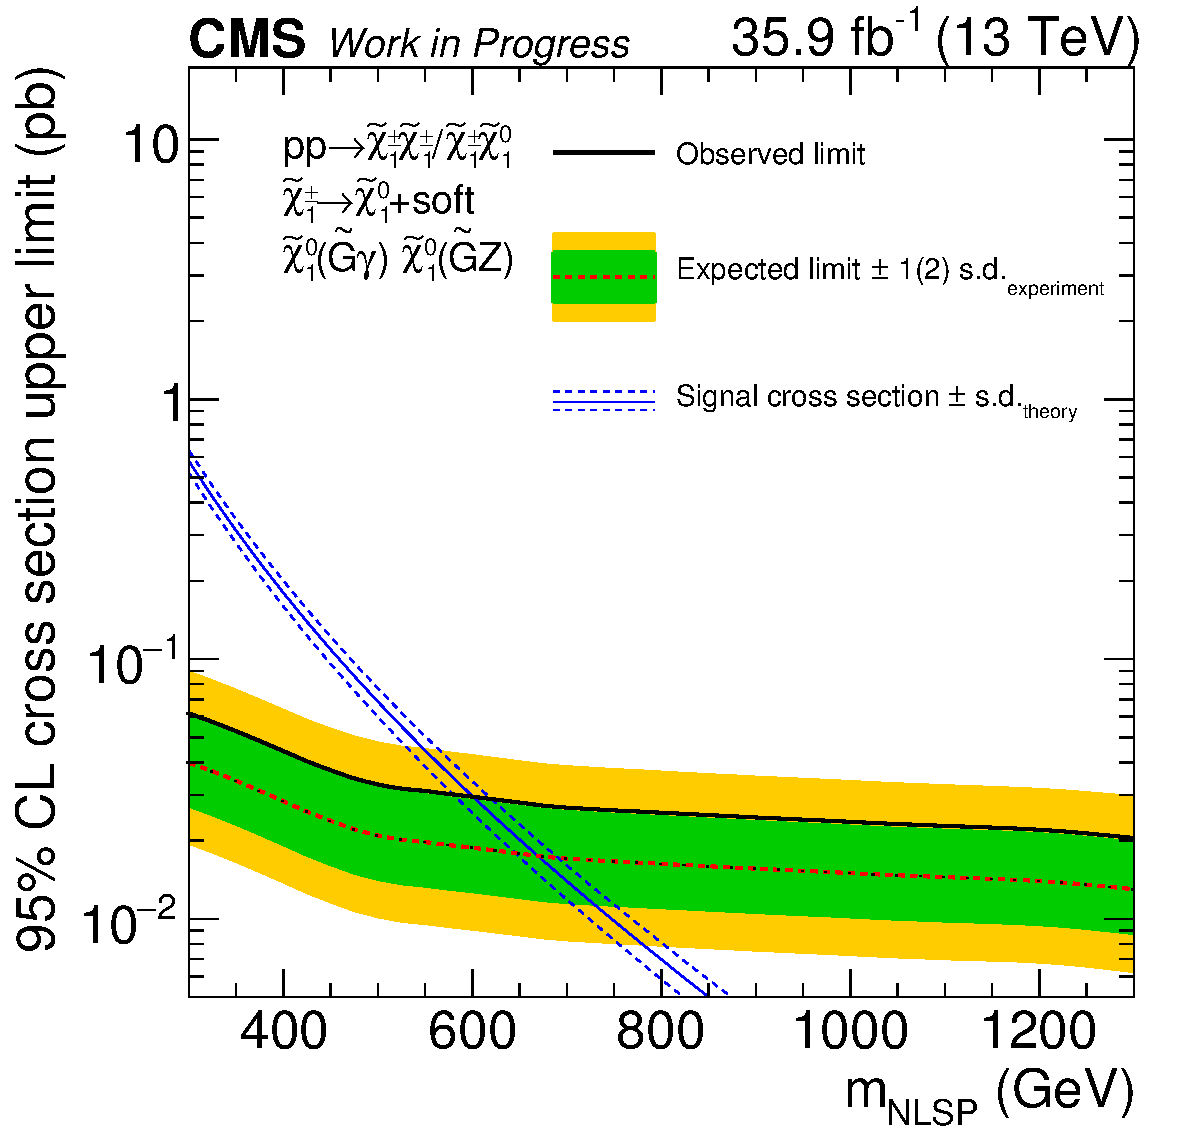
\includegraphics[width=\pairwidth]{figures/UnblindingPlots/TChiNG_limit2}
 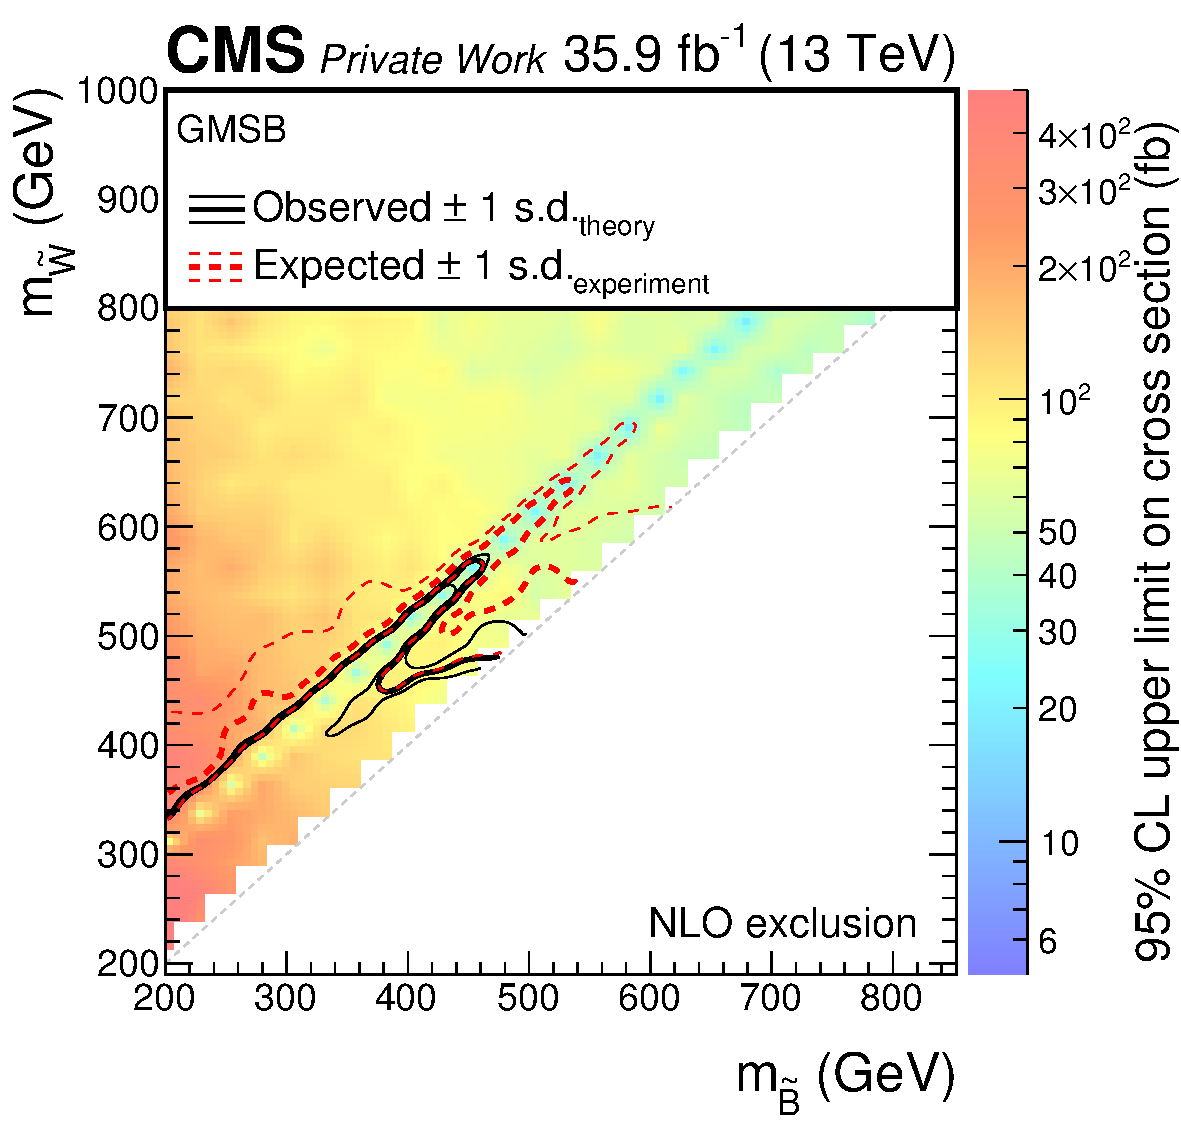
\includegraphics[width=\pairwidth]{figures/UnblindingPlots/GMSB_limits_XSEC2}
 \caption{Expected and observed upper limits for the TChiZG electroweak SMS (left) and the full GMSB model (right).}
 \label{fig:limitEWK}
\end{figure}
Upper cross section limits for the two dimensional GMSB model are shown in \refFig{fig:limitEWK} (right) together with the expected limit contour (red) and the observed limit contour (black). The uncertainty band of the expected limit represents all analysis specific uncertainties, while the uncertainty band of the observed limit reflects theoretical cross section uncertainties. The limits are shown in the wino-bino mass plane, where the wino mass corresponds to the $\charginoOne$ and $\neutralinoTwo$ mass, and the bino mass corresponds to the NLSP $\neutralinoOne$ mass, as discussed in \refSec{sec:SMS}. The analysis has highest sensitivity in cases where the bino and wino mass differ by around $90\GeV$, so that the Z boson production in the decays of the wino is enhanced, as can be seen by the diagonal-like structure in the cross section limit plane. The sensitivity weakens for lower and higher wino masses, since the available energy is split between all decay products. For degenerate bino and wino masses, the sensitivity increases again, because nearly all energy is transferred into the final decay products, the gravitinos and the selected bosons. Due to the cross section increase for larger bino masses, the sensitivity loses there. In total the analysis can exclude bino and wino masses in a range up to $400-500\GeV$ depending on the wino mass.\\
The exclusion contours show the same behavior as for the one dimensional exclusion discussed above, due to the overfluctuation in data in the second SR bin. Therefore, the observed limit is weaker than the expected limit.


\subsubsection*{Limits on strong production of gluinos}
In addition to the limits on EWK SUSY production, the results are interpreted in a SMS with gluino pair production. The cross section upper limits are shown in \refFig{fig:limitStrong} in the gluino-NLSP mass plane.\\
The analysis can exclude gluino masses up to $1.4\TeV$, depending on the mass of the NLSP ($\neutralinoOne$), and thus the mass splitting between them. For NLSP masses lower than the $150\GeV$ the sensitivity drops because of the applied $\mtTwo$ threshold of $100\GeV$ and its poor mass resolution due to the difficulty in the interpretation of $\ptmiss$. With increased $\neutralinoOne$ mass the sensitivity rises, since the final state products carry much more energy than for lower $\neutralinoOne$ masses. Again, the same effect between expected and observed limit contour is observable.

\begin{figure}[tbp]
 \centering
 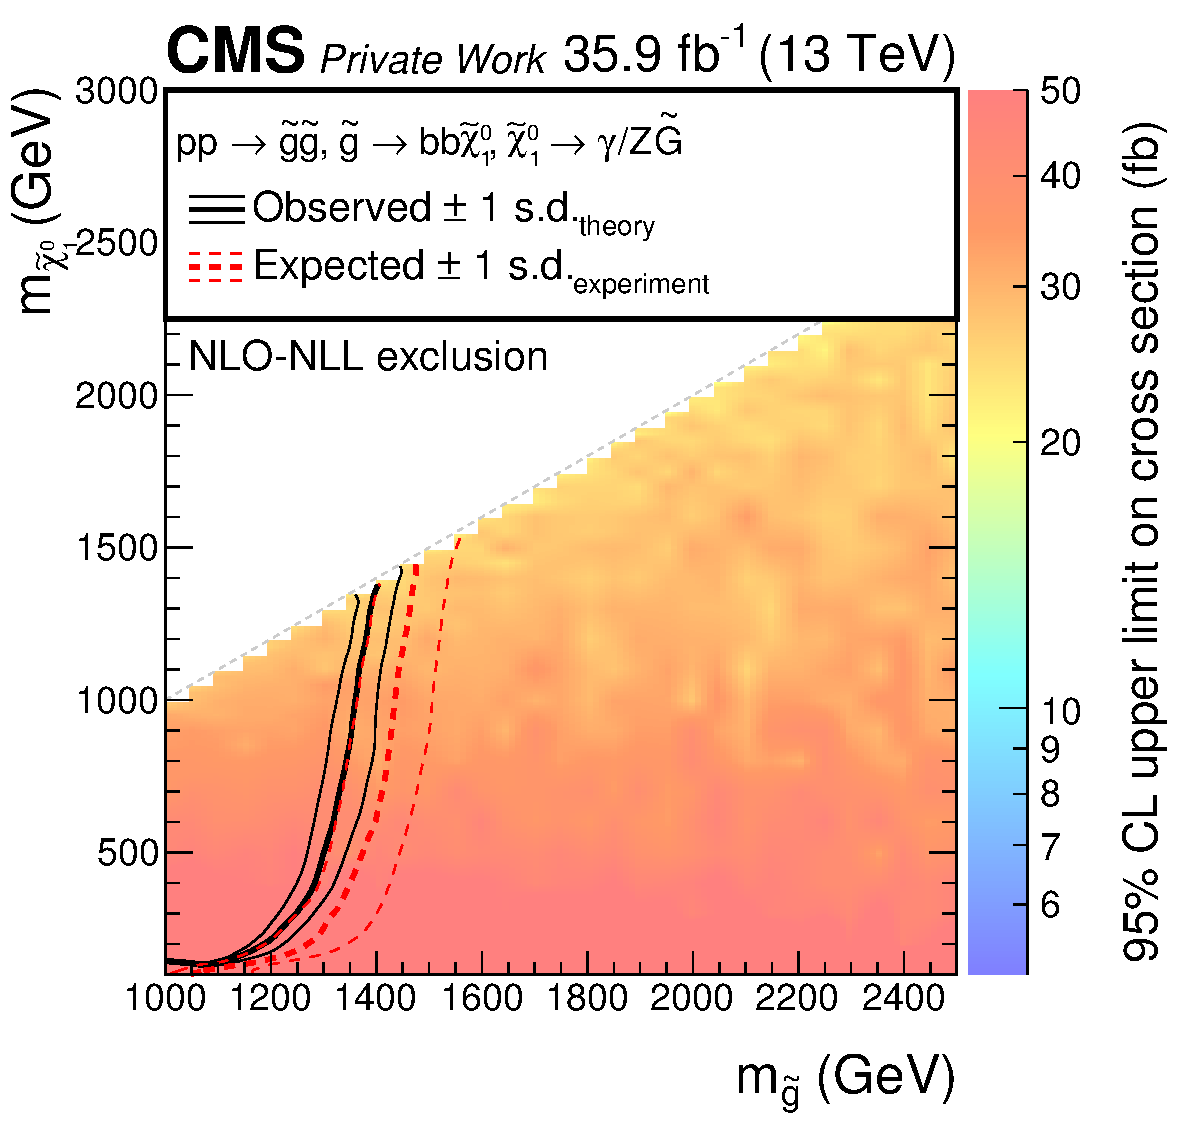
\includegraphics[width=\pairwidth]{figures/UnblindingPlots/T5bbbbZg_limits_XSEC2}
 \caption{Expected and observed upper limits for the T5bbbbZG SMS with strong production.}
 \label{fig:limitStrong}
\end{figure}
